%%%%%%%%%%%%%%%%%%%%%%%%%%%%%%%%%%%%%%%%%%%%%%%%%%%%%%%%%%%%%%%%%%%%%%%%%%%%%%%%
\chapter{Постановка задачи извлечения вопросно-ответных пар}
\label{chap:task}

Цель данной работы~--- разработка алгоритма по извлечению ВОП из обращений в службу поддержки, пригодных для добавления в ЧЗВ. 

Использование такого алгоритма в рабочем процессе технической поддержки позволит:

\begin{enumerate}
\item Упростить заполнение ЧЗВ и документации;
\item Уменьшить количество типовых обращений в службу поддержки;
\item Уделять больше внимания нетривиальным обращениям и задачам.
\end{enumerate}

Команда технической поддержки и команда технических писателей в ручную просматривают весь объем пользовательских обращений с целью, например, найти информацию, актуальную для добавления в FAQ или в раздел по устранению неполадок в  технической документации или для поиска ответа на обращение. Добавление автоматизации в этот процесс упростит содержание ЧЗВ и соответсвующего раздела в документации в актуальном состоянии, что уменьшит количество типовых обращений в ТП и высвободит дополнительные ресурсы для нетривиальных обращений и задач. 

Стоит отметить, что задача не решается полностью автоматически, поскольку текст извлеченных ВОП может содержать, персональные данные или грамматические ошибки. Текст такой вопросно-ответной пары должен быть отредактирован перед публикацией. В связи с чем возникает необходимость проведения экспертного анализа~--- ручного этапа работы. Весь подход при этом является полуавтоматическим.

%%%%%%%%%%%%%%%%%%%%%%%%%%%%%%%%%%%%%%%%%%%%%%%%%%%%%%%%%%%%%%%%%%%%%%%%%%%%%%%%
\section{Анализируемые данные}
\label{sec:data}
%%%%%%%%%%%%%%%%%%%%%%%%%%%%%%%%%%%%%%%%%%%%%%%%%%%%%%%%%%%%%%%%%%%%%%%%%%%%%%%%
В данной работе для анализа использовались обращения пользователей в техническую поддержку системы отслеживания ошибок YouTrack\footnote{http://jetbrains.ru/products/youtrack/}. Для взаимодействия с пользователями команда YouTrack использует Zendesk\footnote{https://www.zendesk.com}~--- систему учета и обработки пользовательских обращений.

\begin{figure}[tph!]
\centerline{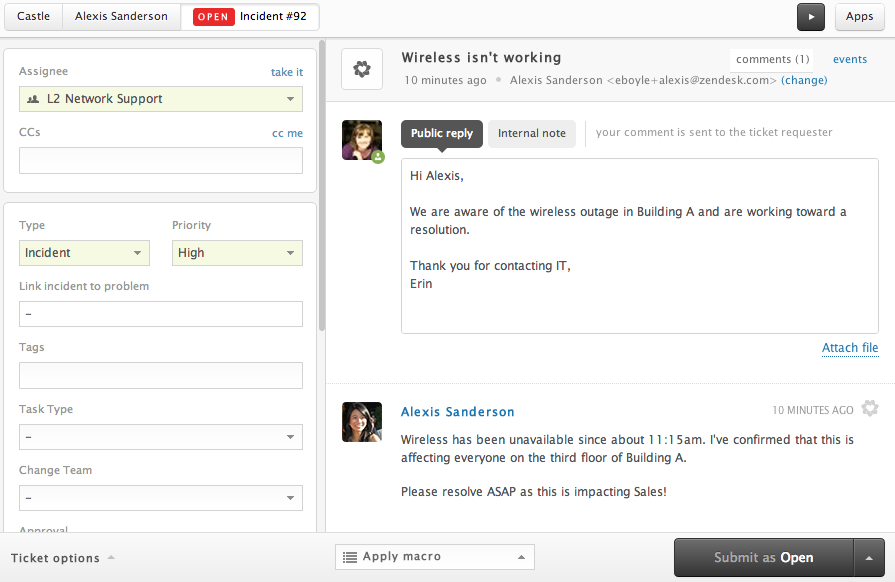
\includegraphics[width=11cm]{fig/zendesk2.png}}
    \caption{Пример обращения в системе Zendesk}
    \label{fig:zdesk_ticket}
\end{figure}

Zendesk позволяет натсраивать различные каналы для получения пользовательских обращений: электронная почта, социальные сети, форма для прямой отправки обращений и так далее. Все собранные таким образом обращения отображаются в едином интерфейсе. На рисунке~\ref{fig:zdesk_ticket} приведен пример обращения в системе Zendesk. 

Обращения состоят из комментариев и, в общем случае, представляют собой диалог между клиентом и сотрудником технической поддержки. Поскольку Zendesk агрегирует все поступающие  обращения, то мы не можем делать предположений о их разбиении по темам. То есть заранее неизвестно, какие из обращений относятся, например, к проблемам администрирования YouTrack, а какие~--- связаны с пользовательским интерфейсом.

В Zendesk каждое обращение содержат ряд метаданных. В то время как использование метаданных ограничивает область применения алгоритма, это позволяет повысить его качество. В данной работе использовалась метаинформация, широко распространенная для данных такого рода: статус обращения и авторство комментария.

Всего в работе анализируются 8500 обращений за период с декабря 2015 года по март 2017 года. 

%%%%%%%%%%%%%%%%%%%%%%%%%%%%%%%%%%%%%%%%%%%%%%%%%%%%%%%%%%%%%%%%%%%%%%%%%%%%%%%%
\section{Формулирвоание требований}
\label{sec:features}
%%%%%%%%%%%%%%%%%%%%%%%%%%%%%%%%%%%%%%%%%%%%%%%%%%%%%%%%%%%%%%%%%%%%%%%%%%%%%%%%

Разрабатываемый алгоритм должен соответствовать следующим требованиям:

\begin{itemize}
\item Приоритет качества над количеством;
\item Обработка только обращений на английском языке;
\item Вопрос и ответ всегда состоят из одного комментария.
\end{itemize}

В работе уделяется большее внимание поиску качественных ВОП (точность), чем поиску всех возможных ВОП (полнота). Основная мотивация такого решения заключается в желании сократить до минимума ручную часть алгоритма~--- валидацию и редактирование ВОП.

Для анализа выбраны обращения на английском языке, поскольку доля таких обращений в техподдержку YouTrack составляет 89\%. 

В качестве ответа всегда выбирается один комментарий. Различные комментарии не комбинируются для составления ответа, поскольку если ответ на вопрос (или сам вопрос) содержатся в более чем одном комментарии, то, вероятно, обращение имеет одну из следующих проблем: вопрос плохо сформулирован, вопрос слишком специфичен или ответ недостаточно полон. Такие ВОП не подходят для добавления в ЧЗВ.

Стоит отметить, что  алгоритм не ограничивается частыми вопросами и позволяет находить редкие ВОП, если они хорошо сформулированы и имеют корректный ответ.

%%%%%%%%%%%%%%%%%%%%%%%%%%%%%%%%%%%%%%%%%%%%%%%%%%%%%%%%%%%%%%%%%%%%%%%%%%%%%%%%
\section{Решаемые задачи}
\label{sec:tasks}
%%%%%%%%%%%%%%%%%%%%%%%%%%%%%%%%%%%%%%%%%%%%%%%%%%%%%%%%%%%%%%%%%%%%%%%%%%%%%%%%

Как было установлено в разделе 1, для извлечения ВОП из большого объема текстовых данных эффективно использовать методы на основе тематического моделирования. В разделе 1 также было установлена наиболее подходящая для данной задачи тематическая модель~--- LDA.

Модель LDA используется для решения похожей задачи в работе~\cite{original}. В статье~\cite{original} решается задача извлечения ВОП из списков рассылки, посвященных различным программным продуктам с открытым исходным кодом. Дополнительно в этой работе применяется ряд эвристик, учитывающих ИТ-тематику анализируемых данных. Воспользуемся этой статьей в качестве опорной.

Далее представлен список решаемых в данной работе задач:

\begin{enumerate}
\item Предобработка данных:
\begin{itemize}
\item Фильтрация обращений;
\item Удаление шумов;
\end{itemize}
\item Кластеризация обращений по тематикам:
\begin{itemize}
\item Тематическое моделирование, LDA;
\end{itemize}
\item Извлечение ВОП:
\begin{itemize}
\item Поиск вопросов;
\item Поиск ответов;
\end{itemize}
\item Тестирование и оценка качества:
\begin{itemize}
\item Экспертный анализ.
\end{itemize}
\end{enumerate}

По сравнению с опорной статьей в текущей работе доработаны и расширены эвристики предобработки данных, применены дополнительные фильтры до и после тематического моделирования. Анализируемые данные~--– обращения в службу технической поддержки~--– никак не размечены, в то время как в статье~\cite{original} тот или иной список рассылки представляет собой заранее известную тему. А также используется перплексия~\cite{LDA} для приблизительного определения количества тем при тематическом моделировании.

Этапы 1--3 подробно рассмотрены в разделах 3 и 4. Тестирование и результаты экспертного анализа приведены в разделе 5.

%%%%%%%%%%%%%%%%%%%%%%%%%%%%%%%%%%%%%%%%%%%%%%%%%%%%%%%%%%%%%%%%%%%%%%%%%%%%%%%%
\section{Резюме}
\label{sec:task_concl}
%%%%%%%%%%%%%%%%%%%%%%%%%%%%%%%%%%%%%%%%%%%%%%%%%%%%%%%%%%%%%%%%%%%%%%%%%%%%%%%%

В данном разеделе были сформулированы требования к разрабатываемому алгоритму. Определены основные этапы разработки, соответсвующие поставленным задачам. Были рассмотрены анализируемые в данной работе данные, которые также используются для тестирования алгоритма.